% Copyright 2006 by Till Tantau
%
% This file may be distributed and/or modified
%
% 1. under the LaTeX Project Public License and/or
% 2. under the GNU Free Documentation License.
%
% See the file doc/generic/pgf/licenses/LICENSE for more details.


\section{Through Library}
\label{section-through-library}

\begin{tikzlibrary}{through}
    This library defines keys for creating shapes that go through given points.
\end{tikzlibrary}
%
\begin{codeexample}[setup code,hidden]
    \usetikzlibrary{through}
\end{codeexample}

\begin{key}{/tikz/circle through=\meta{coordinate}}
    When this key is given as an option to a node, the following happens:
    %
    \begin{enumerate}
        \item The |inner sep| and the |outer sep| are set to zero.
        \item The shape is set to |circle|.
        \item The |minimum size| is set such that the circle around the center
            of the node (which is specified using |at|), goes through
            \meta{coordinate}.
    \end{enumerate}
    %
\begin{codeexample}[]
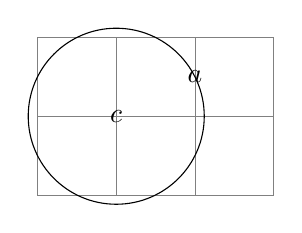
\begin{tikzpicture}
  \draw[help lines] (0,0) grid (3,2);
  \node (a) at (2,1.5) {$a$};
  \node [draw] at (1,1) [circle through={(a)}] {$c$};
\end{tikzpicture}
\end{codeexample}
    %
\end{key}


%%% Local Variables:
%%% mode: latex
%%% TeX-master: "pgfmanual-pdftex-version"
%%% End:
